\section{Preventivo}
È importante tener conto che i periodi di Analisi e Consolidamento dei requisiti sono considerati un investimento per il gruppo e che quindi non sono a carico del Committente\ped{\textit{G}}.
Di conseguenza le ore necessarie allo svolgimento delle attività di questi due periodi saranno conteggiate nel totale delle ore da retribuire. \\

La suddivisione oraria viene fatta rispettando le seguenti regole:
\begin{itemize}
	\item il totale delle ore di lavoro deve essere equamente distribuito tra i componenti del gruppo;
	\item ciascun componente deve ricoprire ogni ruolo almeno una volta;
	\item non si dovranno verificare situazioni nelle quali un Verificatore debba verificare il proprio lavoro.
\end{itemize}

Per semplificare la lettura delle tabelle seguenti verranno utilizzate le seguenti sigle per identificare i ruoli:
\begin{itemize}
	\item \textbf{Rp}: Responsabile di Progetto;
	\item \textbf{As}: Amministratore;
	\item \textbf{An}: Analista;
	\item \textbf{Pt}: Progettista;
	\item \textbf{Pr}: Programmatore;
	\item \textbf{Vf}: Verificatore.
\end{itemize}
Inoltre le celle che contengono un valore pari a 0 presenteranno il simbolo '-'.

\newpage

\subsection{Analisi}
	\subsubsection{Prospetto orario}
		Distribuzione delle ore per ciascun ruolo nel periodo di Analisi:

		\rowcolors{2}{lightRowColor}{darkRowColor}
		\begin{longtable}{
			>{\centering}p{0.25\textwidth}
			>{\centering}p{0.05\textwidth}
			>{\centering}p{0.05\textwidth}
			>{\centering}p{0.05\textwidth}
			>{\centering}p{0.05\textwidth}
			>{\centering}p{0.05\textwidth}
			>{\centering}p{0.05\textwidth}
			>{\centering\arraybackslash}p{0.15\textwidth} }

			\coloredTableHead
			\textbf{\color{white}Nome} &
			\textbf{\color{white}Rp} &
			\textbf{\color{white}As} &
			\textbf{\color{white}An} &
			\textbf{\color{white}Pt} &
			\textbf{\color{white}Pr} &
			\textbf{\color{white}Vf} &
			\textbf{\color{white}Totale}
			\tabularnewline
			\endhead

			% Contenuto della tabella
			% Nome & Rp & As & An & Pt & Pr & Vf & Totale \\
			\VB & 10 & 20 & -  & -  & - & -  & 30 \\
			\LB & -  & 20 & -  & -  & - & 10 & 30 \\
			\NF & -  & 20 & -  & 10 & - & -  & 30 \\
			\EG & -  & 5  & 30 & -  & - & -  & 35 \\
			\FJ & -  & -  & -  & 10 & - & 20 & 30 \\
			\MP & 20 & -  & -  & -  & - & 10 & 30 \\
			\AS & -  & 5  & -  & -  & - & 25 & 30 \\
			\AZ & -  & -  & 30 & -  & - & 5  & 35 \\
			\textbf{Ore totali per ruolo} & 30 & 70 & 60 & 20 & - & 70 & 250 \\

			\rowcolor{white}\caption{Suddivisione oraria del periodo di Analisi}	\\

		\end{longtable}

		% Grafico
		Rappresentazione grafica della suddivisione oraria:
		\begin{figure}[h]
			\centering
			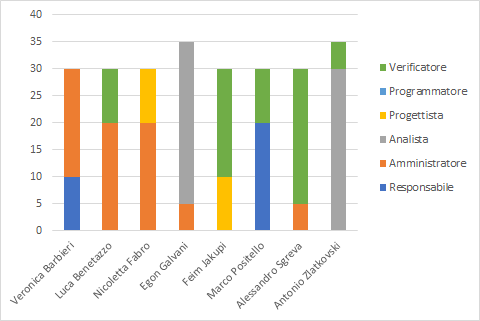
\includegraphics[width=0.7\textwidth]{./res/img/analisi_po.png}
			\caption{Suddivisione oraria del periodo di Analisi}
		\end{figure}

	\newpage
	\subsubsection{Prospetto economico}
		Totale delle ore e costo per ciascun ruolo nel periodo di Analisi:

		\rowcolors{2}{lightRowColor}{darkRowColor}
		\begin{longtable}{
			>{\centering}p{0.25\textwidth}
			>{\centering}p{0.05\textwidth}
			>{\centering\arraybackslash}p{0.15\textwidth} }

			\coloredTableHead
			\textbf{\color{white}Ruolo} &
			\textbf{\color{white}Ore} &
			\textbf{\color{white}Costo in \euro{}}
			\tabularnewline
			\endhead

			% Contenuto della tabella
			% Ruolo & Ore & Costo\\
			Responsabile    & 30  & 900,00 \\
			Amministratore  & 70  & 1.400,00 \\
			Analista        & 60  & 1.500,00 \\
			Progettista     & 20  & 440,00 \\
			Programmatore   & -   & - \\
			Verificatore    & 70  & 1.050,00 \\
			\textbf{Totale} & 250 & 5.290,00 \\

			\rowcolor{white}\caption{Prospetto dei costi per il periodo di Analisi}	\\

		\end{longtable}

		% Grafico
		Rappresentazione grafica della distribuzione dei ruoli:
		\begin{figure}[h]
			\centering
			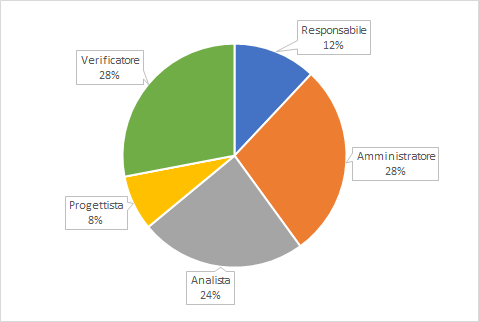
\includegraphics[width=0.7\textwidth]{./res/img/analisi_pe.png}
			\caption{Suddivisione dei ruoli nel periodo di Analisi}
		\end{figure}

\newpage
\subsection{Consolidamento dei Requisiti}
	\subsubsection{Prospetto orario}
		Distribuzione delle ore per ciascun ruolo nel periodo di Consolidamento dei requisiti:

		\rowcolors{2}{lightRowColor}{darkRowColor}
		\begin{longtable}{
			>{\centering}p{0.25\textwidth}
			>{\centering}p{0.05\textwidth}
			>{\centering}p{0.05\textwidth}
			>{\centering}p{0.05\textwidth}
			>{\centering}p{0.05\textwidth}
			>{\centering}p{0.05\textwidth}
			>{\centering}p{0.05\textwidth}
			>{\centering\arraybackslash}p{0.15\textwidth} }

			\coloredTableHead
			\textbf{\color{white}Nome} &
			\textbf{\color{white}Rp} &
			\textbf{\color{white}As} &
			\textbf{\color{white}An} &
			\textbf{\color{white}Pt} &
			\textbf{\color{white}Pr} &
			\textbf{\color{white}Vf} &
			\textbf{\color{white}Totale}
			\tabularnewline
			\endhead

			% Contenuto della tabella
			% Nome & Rp & As & An & Pt & Pr & Vf & Totale \\
			\VB & - & - & 3 & - & - & 2 & 5 \\
			\LB & 5 & - & - & - & - & - & 5 \\
			\NF & - & - & - & - & - & 5 & 5 \\
			\EG & - & 3 & - & - & - & - & 3 \\
			\FJ & - & - & 3 & - & - & 2 & 5 \\
			\MP & - & - & 2 & - & - & 3 & 5 \\
			\AS & - & - & 2 & - & - & 3 & 5 \\
			\AZ & - & 3 & - & - & - & - & 3 \\
			\textbf{Ore totali per ruolo} & 5 & 6 & 10 & - & - & 15 & 36 \\

			\rowcolor{white}\caption {Suddivisione oraria del periodo di Consolidamento dei requisiti} \\

		\end{longtable}

		% Grafico
		Rappresentazione grafica della suddivisione oraria:
		\begin{figure}[h]
			\centering
			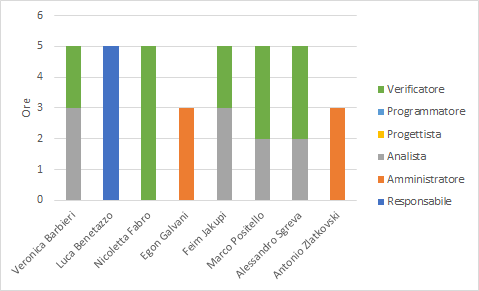
\includegraphics[width=0.7\textwidth]{./res/img/consolidamentoRequisiti_po.png}
			\caption{Suddivisione oraria del periodo di Consolidamento dei requisiti}
		\end{figure}

	\newpage
	\subsubsection{Prospetto economico}
		Totale delle ore e costo per ciascun ruolo nel periodo di Consolidamento dei requisiti:

		\rowcolors{2}{lightRowColor}{darkRowColor}
		\begin{longtable}{
			>{\centering}p{0.25\textwidth}
			>{\centering}p{0.05\textwidth}
			>{\centering\arraybackslash}p{0.15\textwidth} }

			\coloredTableHead
			\textbf{\color{white}Ruolo} &
			\textbf{\color{white}Ore} &
			\textbf{\color{white}Costo in \euro{}}
			\tabularnewline
			\endhead

			% Contenuto della tabella
			% Ruolo & Ore & Costo \\
			Responsabile    & 5  & 150,00 \\
			Amministratore  & 6  & 120,00 \\
			Analista        & 10 & 250,00 \\
			Progettista     & -  & - \\
			Programmatore   & -  & - \\
			Verificatore    & 15 & 225,00 \\
			\textbf{Totale} & 36 & 745,00 \\

			\rowcolor{white}\caption {Prospetto dei costi per il periodo di Consolidamento dei requisiti}	\\

		\end{longtable}

		% Grafico
		Rappresentazione grafica della distribuzione dei ruoli:
		\begin{figure}[h]
			\centering
			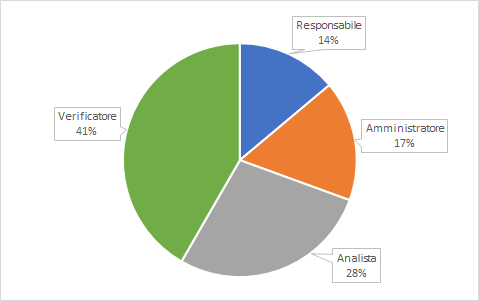
\includegraphics[width=0.7\textwidth]{./res/img/consolidamentoRequisiti_pe.png}
			\caption{Suddivisione dei ruoli nel periodo di Consolidamento dei requisiti}
		\end{figure}

\newpage
\subsection{Progettazione Architetturale}
	\subsubsection{Prospetto orario}
		Distribuzione delle ore per ciascun ruolo nel periodo di Progettazione architetturale:

		\rowcolors{2}{lightRowColor}{darkRowColor}
		\begin{longtable}{
			>{\centering}p{0.25\textwidth}
			>{\centering}p{0.05\textwidth}
			>{\centering}p{0.05\textwidth}
			>{\centering}p{0.05\textwidth}
			>{\centering}p{0.05\textwidth}
			>{\centering}p{0.05\textwidth}
			>{\centering}p{0.05\textwidth}
			>{\centering\arraybackslash}p{0.15\textwidth} }

			\coloredTableHead
			\textbf{\color{white}Nome} &
			\textbf{\color{white}Rp} &
			\textbf{\color{white}As} &
			\textbf{\color{white}An} &
			\textbf{\color{white}Pt} &
			\textbf{\color{white}Pr} &
			\textbf{\color{white}Vf} &
			\textbf{\color{white}Totale}
			\tabularnewline
			\endhead

			% Contenuto della tabella
			% Nome & Rp & As & An & Pt & Pr & Vf & Totale \\
			\VB & - & -  & -  & 8  & 7 & 16 & 31 \\
			\LB & 5 & -  & 10 & 11 & 5 & -  & 31 \\
			\NF & - & -  & 6  & 15 & - & 10 & 31 \\
			\EG & - & -  & 7  & 8  & 6 & 10 & 31 \\
			\FJ & - & 6  & -  & 8  & 7 & 10 & 31 \\
			\MP & - & 8  & -  & 15 & - & 8  & 31 \\
			\AS & - & 10 & -  & 7  & 6 & 8  & 31 \\
			\AZ & 7 & -  & 10 & -  & 8 & 6  & 31 \\
			\textbf{Ore totali per ruolo} & 12 & 24 & 33 & 72 & 39 & 68 & 248 \\

			\rowcolor{white}\caption {Suddivisione oraria del periodo di Progettazione architetturale} \\

		\end{longtable}

		% Grafico
		\begin{figure}[h]
			\centering
			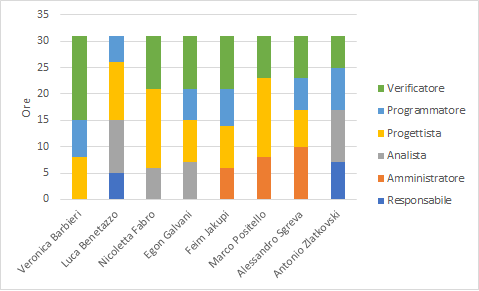
\includegraphics[width=0.7\textwidth]{./res/img/progettazioneArchitetturale_po.png}
			\caption{Suddivisione oraria del periodo di Progettazione architetturale}
		\end{figure}

		\newpage
		\subsubsection{Pianificazione oraria interna agli incrementi}
		\rowcolors{2}{lightRowColor}{darkRowColor}
		\begin{longtable}{
			>{\centering}p{0.25\textwidth}
			>{\centering}p{0.05\textwidth}
			>{\centering}p{0.05\textwidth}
			>{\centering}p{0.05\textwidth}
			>{\centering}p{0.05\textwidth}
			>{\centering}p{0.05\textwidth}
			>{\centering}p{0.05\textwidth}
			>{\centering\arraybackslash}p{0.10\textwidth}
			>{\centering\arraybackslash}p{0.10\textwidth} }

			\coloredTableHead
			\textbf{\color{white}Incremento} &
			\textbf{\color{white}Rp} &
			\textbf{\color{white}As} &
			\textbf{\color{white}An} &
			\textbf{\color{white}Pt} &
			\textbf{\color{white}Pr} &
			\textbf{\color{white}Vf} &
			\textbf{\color{white}Totale ore} &
			\textbf{\color{white}Totale \euro{}}
			\tabularnewline
			\endhead

			% Contenuto della tabella
			% n'Incr & Rp & As & An & Pt & Pr & Vf & Totale Ore \\
			1' Incremento & 2 & 5  & 11 & 7  & -  & 11 & 35 & 754,00\\
			2' Incremento & 1 & 5  & 8  & 12 & 9  & 8  & 43 & 849,00\\
			3' Incremento & 1 & 3  & 3  & 14 & 10 & 8  & 39 & 743,00\\
			4' Incremento & 1 & 3  & 3  & 14 & 10 & 8  & 39 & 743,00\\
			5' Incremento & 2 & 3  & 3  & 12 & 10 & 7  & 37 & 714,00\\
			6' Incremento & 2 & 3  & 4  & 7  & -  & 13 & 29 & 569,00\\
			7' Incremento & 2 & 1  & 1  & 6  & -  & 11 & 21 & 402,00\\
			8' Incremento & 1 & 1  & -  & -  & -  & 2  & 4  & 80,00\\
			\textbf{Ore e costo totali} & 12 & 24 & 33 & 72 & 39 & 68 & 248 & 4.854,00 \\

			\rowcolor{white}\caption {Suddivisione oraria per incremento del periodo di Progettazione architetturale} \\

		\end{longtable}

	\subsubsection{Prospetto economico}
		Totale delle ore e costo per ciascun ruolo nel periodo di Progettazione architetturale:

		\rowcolors{2}{lightRowColor}{darkRowColor}
		\begin{longtable}{
			>{\centering}p{0.25\textwidth}
			>{\centering}p{0.05\textwidth}
			>{\centering\arraybackslash}p{0.15\textwidth} }

			\coloredTableHead
			\textbf{\color{white}Ruolo} &
			\textbf{\color{white}Ore} &
			\textbf{\color{white}Costo in \euro{}}
			\tabularnewline
			\endhead

			% Contenuto della tabella
			% Ruolo & Ore & Costo \\
			Responsabile    & 12  & 360,00 \\
			Amministratore  & 24  & 480,00 \\
			Analista        & 33  & 825,00 \\
			Progettista     & 72  & 1.584,00 \\
			Programmatore   & 39  & 585,00 \\
			Verificatore    & 68  & 1.020,00 \\
			\textbf{Totale} & 248 & 4.854,00 \\

			\rowcolor{white}\caption {Prospetto dei costi per il periodo di Progettazione architetturale}	\\

		\end{longtable}

		% Grafico
		Rappresentazione grafica della distribuzione dei ruoli:
		\begin{figure}[h]
			\centering
			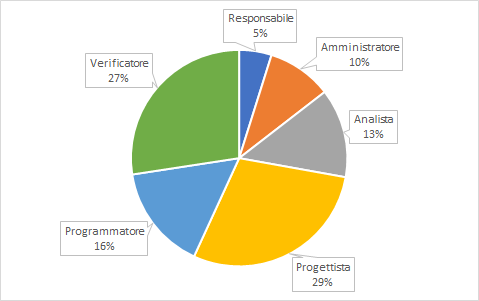
\includegraphics[width=0.7\textwidth]{./res/img/progettazioneArchitetturale_pe.png}
			\caption{Suddivisione dei ruoli nel periodo di Progettazione architetturale}
		\end{figure}

\newpage
\subsection{Progettazione di Dettaglio e Codifica}
	\subsubsection{Prospetto orario}
	Distribuzione delle ore per ciascun ruolo nel periodo di Progettazione di dettaglio e codifica:

		\rowcolors{2}{lightRowColor}{darkRowColor}
		\begin{longtable}{
			>{\centering}p{0.25\textwidth}
			>{\centering}p{0.05\textwidth}
			>{\centering}p{0.05\textwidth}
			>{\centering}p{0.05\textwidth}
			>{\centering}p{0.05\textwidth}
			>{\centering}p{0.05\textwidth}
			>{\centering}p{0.05\textwidth}
			>{\centering\arraybackslash}p{0.15\textwidth} }

			\coloredTableHead
			\textbf{\color{white}Nome} &
			\textbf{\color{white}Rp} &
			\textbf{\color{white}As} &
			\textbf{\color{white}An} &
			\textbf{\color{white}Pt} &
			\textbf{\color{white}Pr} &
			\textbf{\color{white}Vf} &
			\textbf{\color{white}Totale}
			\tabularnewline
			\endhead

			% Contenuto della tabella
			% Nome & Rp & As & An & Pt & Pr & Vf & Totale \\
			\VB & 7 & 4 & - & 6  & 20 & 12 & 49 \\
			\LB & - & - & - & 15 & 20 & 14 & 49 \\
			\NF & - & 8 & - & 12 & 19 & 10 & 49 \\
			\EG & 6 & - & - & 15 & 20 & 8  & 49 \\
			\FJ & 5 & 5 & - & 10 & 19 & 10 & 49 \\
			\MP & 5 & 6 & - & 8  & 15 & 15 & 49 \\
			\AS & - & - & - & 14 & 20 & 15 & 49 \\
			\AZ & - & 9 & - & 8  & 20 & 12 & 49 \\
			\textbf{Ore totali per ruolo} & 23 & 32 & - & 88 & 153 & 96 & 392 \\

			\rowcolor{white}\caption {Suddivisione oraria del periodo di Progettazione di dettaglio e codifica} \\

		\end{longtable}

		\newpage
		% Grafico
		Rappresentazione grafica della suddivisione oraria:
		\begin{figure}[h]
			\centering
			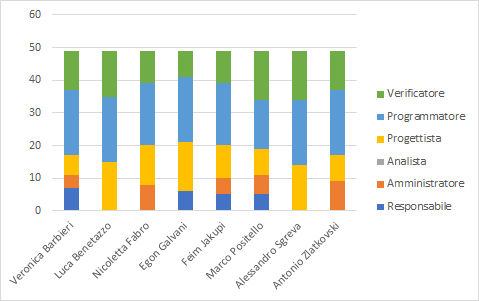
\includegraphics[width=0.7\textwidth]{./res/img/progettazioneDettaglioCodifica_po.png}
			\caption{Suddivisione oraria del periodo di Progettazione di dettaglio e codifica}
		\end{figure}

		\subsubsection{Pianificazione oraria interna agli incrementi}
		\rowcolors{2}{lightRowColor}{darkRowColor}
		\begin{longtable}{
			>{\centering}p{0.25\textwidth}
			>{\centering}p{0.05\textwidth}
			>{\centering}p{0.05\textwidth}
			>{\centering}p{0.05\textwidth}
			>{\centering}p{0.05\textwidth}
			>{\centering}p{0.05\textwidth}
			>{\centering}p{0.05\textwidth}
			>{\centering\arraybackslash}p{0.10\textwidth}
			>{\centering\arraybackslash}p{0.10\textwidth} }

			\coloredTableHead
			\textbf{\color{white}Incremento} &
			\textbf{\color{white}Rp} &
			\textbf{\color{white}As} &
			\textbf{\color{white}An} &
			\textbf{\color{white}Pt} &
			\textbf{\color{white}Pr} &
			\textbf{\color{white}Vf} &
			\textbf{\color{white}Totale ore} &
			\textbf{\color{white}Totale \euro{}}
			\tabularnewline
			\endhead

			% Contenuto della tabella
			% n'Incr & Rp & As & An & Pt & Pr & Vf & Totale Ore \\
			1' Incremento & 2 & 8 & - & 10 & -  & 17 & 37 & 695,00\\
			2' Incremento & 6 & 4 & - & 35 & 27 & 25 & 97 & 1.810,00\\
			3' Incremento & 5 & 7 & - & 15 & 50 & 15 & 92 & 1.595,00\\
			4' Incremento & 5 & 7 & - & 23 & 75 & 30 & 39 & 2.371,00\\
			5' Incremento & 3 & 4 & - & 3  & 1  & 1  & 16 & 319,00\\
			6' Incremento & 2 & 2 & - & 3  & 1  & 1  & 10 & 211,00\\
			\textbf{Ore e costo totali} & 23 & 32 & - & 88 & 153 & 96 & 392 & 7.001,00 \\

			\rowcolor{white}\caption {Suddivisione oraria per incremento del periodo di Progettazione di Dettaglio e Codifica} \\

		\end{longtable}

	\newpage
	\subsubsection{Prospetto economico}
		Totale delle ore e costo per ciascun ruolo nel periodo di Progettazione di dettaglio e codifica:

		\rowcolors{2}{lightRowColor}{darkRowColor}
		\begin{longtable}{
			>{\centering}p{0.25\textwidth}
			>{\centering}p{0.05\textwidth}
			>{\centering\arraybackslash}p{0.15\textwidth} }

			\coloredTableHead
			\textbf{\color{white}Ruolo} &
			\textbf{\color{white}Ore} &
			\textbf{\color{white}Costo in \euro{}}
			\tabularnewline
			\endhead

			% Contenuto della tabella
			% Ruolo & Ore & Costo \\
			Responsabile    & 23 & 690,00 \\
			Amministratore  & 32 & 640,00 \\
			Analista        & -  & - \\
			Progettista     & 88 & 1.936,00 \\
			Programmatore   & 153 & 2.295,00 \\
			Verificatore    & 96  & 1.440,00 \\
			\textbf{Totale} & 392 & 7.001,00 \\

			\rowcolor{white}\caption {Prospetto dei costi per il periodo di Progettazione di dettaglio e codifica} \\

		\end{longtable}

		% Grafico
		Rappresentazione grafica della distribuzione dei ruoli:
		\begin{figure}[h]
			\centering
			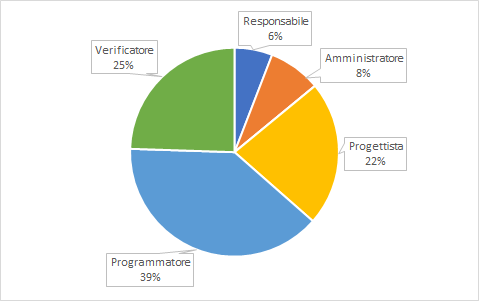
\includegraphics[width=0.7\textwidth]{./res/img/progettazioneDettaglioCodifica_pe.png}
			\caption{Suddivisione dei ruoli nel periodo di Progettazione di dettaglio e codifica}
		\end{figure}

\newpage
\subsection{Validazione e Collaudo}
	\subsubsection{Prospetto orario}
	Distribuzione delle ore per ciascun ruolo nel periodo di Validazione e collaudo:

		\rowcolors{2}{lightRowColor}{darkRowColor}
		\begin{longtable}{
			>{\centering}p{0.25\textwidth}
			>{\centering}p{0.05\textwidth}
			>{\centering}p{0.05\textwidth}
			>{\centering}p{0.05\textwidth}
			>{\centering}p{0.05\textwidth}
			>{\centering}p{0.05\textwidth}
			>{\centering}p{0.05\textwidth}
			>{\centering\arraybackslash}p{0.15\textwidth} }

			\coloredTableHead
			\textbf{\color{white}Nome} &
			\textbf{\color{white}Rp} &
			\textbf{\color{white}As} &
			\textbf{\color{white}An} &
			\textbf{\color{white}Pt} &
			\textbf{\color{white}Pr} &
			\textbf{\color{white}Vf} &
			\textbf{\color{white}Totale}
			\tabularnewline
			\endhead

			% Contenuto della tabella
			% Nome & Rp & As & An & Pt & Pr & Vf & Totale \\
			\VB & - & - & - & 5 & 7  & 10 & 22 \\
			\LB & - & 6 & - & - & 10 & 6  & 22 \\
			\NF & 5 & - & - & - & 7  & 10 & 22 \\
			\EG & - & 5 & - & 7 & -  & 10 & 22 \\
			\FJ & 6 & 6 & - & - & 5  & 5  & 22 \\
			\MP & 5 & - & - & - & 7  & 10 & 22 \\
			\AS & 6 & - & - & - & 5  & 11 & 22 \\
			\AZ & - & - & - & 6 & 6  & 10 & 22 \\
			\textbf{Ore totali per ruolo} & 22 & 17 & - & 18 & 47 & 72 & 176 \\

			\rowcolor{white}\caption {Suddivisione oraria del periodo di Validazione e collaudo} \\

		\end{longtable}

		% Grafico
		Rappresentazione grafica della suddivisione oraria:
		\begin{figure}[h]
			\centering
			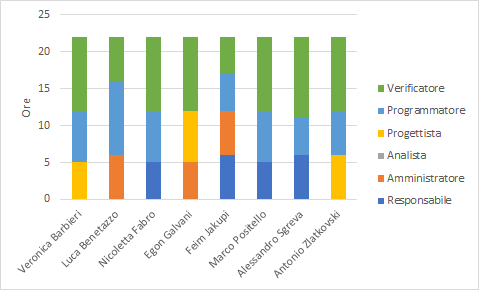
\includegraphics[width=0.7\textwidth]{./res/img/validazioneCollaudo_po.png}
			\caption{Suddivisione oraria del periodo di Validazione e collaudo}
		\end{figure}

		\newpage
		\subsubsection{Pianificazione oraria interna agli incrementi}
		\rowcolors{2}{lightRowColor}{darkRowColor}
		\begin{longtable}{
			>{\centering}p{0.25\textwidth}
			>{\centering}p{0.05\textwidth}
			>{\centering}p{0.05\textwidth}
			>{\centering}p{0.05\textwidth}
			>{\centering}p{0.05\textwidth}
			>{\centering}p{0.05\textwidth}
			>{\centering}p{0.05\textwidth}
			>{\centering\arraybackslash}p{0.10\textwidth}
			>{\centering\arraybackslash}p{0.10\textwidth} }

			\coloredTableHead
			\textbf{\color{white}Incremento} &
			\textbf{\color{white}Rp} &
			\textbf{\color{white}As} &
			\textbf{\color{white}An} &
			\textbf{\color{white}Pt} &
			\textbf{\color{white}Pr} &
			\textbf{\color{white}Vf} &
			\textbf{\color{white}Totale ore} &
			\textbf{\color{white}Totale \euro{}}
			\tabularnewline
			\endhead

			% Contenuto della tabella
			% n'Incr & Rp & As & An & Pt & Pr & Vf & Totale Ore \\
			1' Incremento & 7 & 6 & - & 3 & 5 & 9 & 30 & 606,00\\
			2' Incremento & 3 & 3 & - & 7 & 23 & 25 & 61 & 1.024,00\\
			3' Incremento & 3 & 3 & - & 4 & 16 & 22 & 48 & 808,00\\
			4' Incremento & 7 & 4 & - & 3 & 2 & 14 & 30 & 596,00\\
			5' Incremento & 2 & 1 & - & 1 & 1 & 2 & 7 & 147,00\\
			\textbf{Ore e costo totali} & 22 & 17 & - & 18 & 47 & 72 & 176 & 3.181,00 \\

			\rowcolor{white}\caption {Suddivisione oraria per incremento del periodo di Validazione e collaudo} \\

		\end{longtable}

	\subsubsection{Prospetto economico}
		Totale delle ore e costo per ciascun ruolo nel periodo di Validazione e collaudo:

		\rowcolors{2}{lightRowColor}{darkRowColor}
		\begin{longtable}{
			>{\centering}p{0.25\textwidth}
			>{\centering}p{0.05\textwidth}
			>{\centering\arraybackslash}p{0.15\textwidth} }

			\coloredTableHead
			\textbf{\color{white}Ruolo} &
			\textbf{\color{white}Ore} &
			\textbf{\color{white}Costo in \euro{}}
			\tabularnewline
			\endhead

			% Contenuto della tabella
			% Ruolo & Ore & Costo in \\
			Responsabile    & 22  & 660,00 \\
			Amministratore  & 17  & 340,00 \\
			Analista        & -   & - \\
			Progettista     & 18  & 396,00 \\
			Programmatore   & 47  & 705,00 \\
			Verificatore    & 72  & 1.080,00 \\
			\textbf{Totale} & 176 & 3.181,00 \\

			\rowcolor{white}\caption {Prospetto dei costi per il periodo di Validazione e collaudo} \\

		\end{longtable}

		\newpage
		% Grafico
		Rappresentazione grafica della distribuzione dei ruoli:
		\begin{figure}[h]
			\centering
			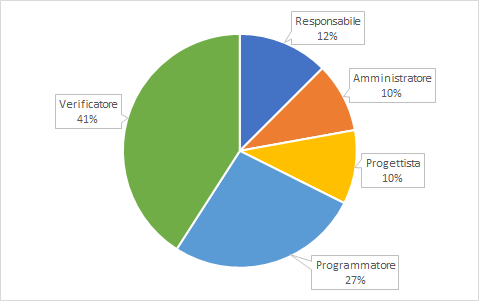
\includegraphics[width=0.7\textwidth]{./res/img/validazioneCollaudo_pe.png}
			\caption{Suddivisione dei ruoli nel periodo di Validazione e collaudo}
		\end{figure}

\subsection{Riepilogo}
	\subsubsection{Ore totali}
		\subsubsubsection{Suddivisione del lavoro}
			Distribuzione totale delle ore per ciascun ruolo comprensive delle ore di investimento e delle ore rendicontate al carico del Committente\ped{\textit{G}}.

			\rowcolors{2}{lightRowColor}{darkRowColor}
			\begin{longtable}{
				>{\centering}p{0.25\textwidth}
				>{\centering}p{0.05\textwidth}
				>{\centering}p{0.05\textwidth}
				>{\centering}p{0.05\textwidth}
				>{\centering}p{0.05\textwidth}
				>{\centering}p{0.05\textwidth}
				>{\centering}p{0.05\textwidth}
				>{\centering\arraybackslash}p{0.15\textwidth} }

				\coloredTableHead
				\textbf{\color{white}Nome} &
				\textbf{\color{white}Rp} &
				\textbf{\color{white}As} &
				\textbf{\color{white}An} &
				\textbf{\color{white}Pt} &
				\textbf{\color{white}Pr} &
				\textbf{\color{white}Vf} &
				\textbf{\color{white}Totale}
				\tabularnewline
				\endhead

				% Contenuto della tabella
				% Nome & Rp & As & An & Pt & Pr & Vf & Totale \\
				\VB & 17 & 24 & 3  & 19 & 34 & 40 & 137 \\
				\LB & 10 & 26 & 10 & 26 & 35 & 30 & 137 \\
				\NF & 5  & 28 & 6  & 37 & 26 & 35 & 137 \\
				\EG & 6  & 13 & 37 & 30 & 26 & 28 & 140 \\
				\FJ & 11 & 17 & 3  & 28 & 31 & 47 & 137 \\
				\MP & 30 & 14 & 2  & 23 & 22 & 46 & 137 \\
				\AS & 6  & 15 & 2  & 21 & 31 & 62 & 137 \\
				\AZ & 7  & 12 & 40 & 14 & 34 & 33 & 140 \\
				\textbf{Ore totali per ruolo} & 92 & 149 & 103 & 198 & 239 & 321 & 1102 \\

				\rowcolor{white}\caption {Suddivisione oraria con il totale delle ore di investimento e rendicontate}	\\

			\end{longtable}

			\newpage
			% Grafico
			Rappresentazione grafica della suddivisione oraria:
			\begin{figure}[h]
				\centering
				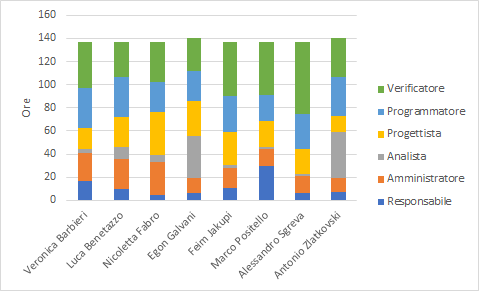
\includegraphics[width=0.7\textwidth]{./res/img/totale_po.png}
				\caption{Suddivisione oraria con il totale delle ore di investimento e rendicontate}
			\end{figure}

		\subsubsubsection{Prospetto econimico}
			Totale delle ore e costo per ciascun ruolo comprensivo delle ore di investimento e delle ore rendicontate a carico del Committente\ped{\textit{G}}:

			\rowcolors{2}{lightRowColor}{darkRowColor}
			\begin{longtable}{
				>{\centering}p{0.25\textwidth}
				>{\centering}p{0.05\textwidth}
				>{\centering\arraybackslash}p{0.15\textwidth} }

				\coloredTableHead
				\textbf{\color{white}Ruolo} &
				\textbf{\color{white}Ore} &
				\textbf{\color{white}Costo in \euro{}}
				\tabularnewline
				\endhead

				% Contenuto della tabella
				% Ruolo & Ore & Costo in \\
				Responsabile    & 92   & 2.760,00 \\
				Amministratore  & 149  & 2.980,00 \\
				Analista        & 103  & 2.575,00 \\
				Progettista     & 198  & 4.356,00 \\
				Programmatore   & 239  & 3.585,00 \\
				Verificatore    & 321  & 4.815,00 \\
				\textbf{Totale} & 1102 & 21.071,00 \\

				\rowcolor{white}\caption {Prospetto dei costi totale delle ore di investimento e rendicontate per ciascun ruolo} \\

			\end{longtable}

			\newpage
			% Grafico
			Rappresentazione grafica della distribuzione dei ruoli:
			\begin{figure}[h]
				\centering
				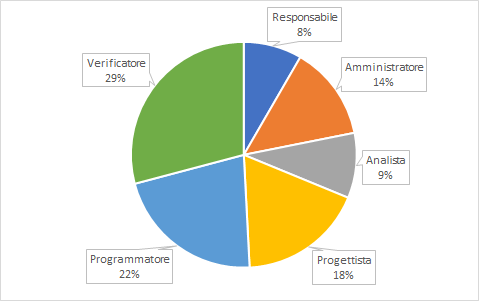
\includegraphics[width=0.7\textwidth]{./res/img/totale_pe.png}
				\caption{Suddivisione dei ruoli per il totale delle ore di investimento e rendicontate }
			\end{figure}

	\subsubsection{Ore rendicontate}
		\subsubsubsection{Suddivisione del lavoro}
			Distribuzione totale delle ore rendicontate per ciascun ruolo.

			\rowcolors{2}{lightRowColor}{darkRowColor}
			\begin{longtable}{
				>{\centering}p{0.25\textwidth}
				>{\centering}p{0.05\textwidth}
				>{\centering}p{0.05\textwidth}
				>{\centering}p{0.05\textwidth}
				>{\centering}p{0.05\textwidth}
				>{\centering}p{0.05\textwidth}
				>{\centering}p{0.05\textwidth}
				>{\centering\arraybackslash}p{0.15\textwidth} }

				\coloredTableHead
				\textbf{\color{white}Nome} &
				\textbf{\color{white}Rp} &
				\textbf{\color{white}As} &
				\textbf{\color{white}An} &
				\textbf{\color{white}Pt} &
				\textbf{\color{white}Pr} &
				\textbf{\color{white}Vf} &
				\textbf{\color{white}Totale}
				\tabularnewline
				\endhead

				% Contenuto della tabella
				% Nome & Rp & As & An & Pt & Pr & Vf & Totale \\
				\VB & 7  & 4  & -  & 19 & 34 & 38 & 102 \\
				\LB & 5  & 6  & 10 & 26 & 35 & 20 & 102 \\
				\NF & 5  & 8  & 6  & 27 & 26 & 30 & 102 \\
				\EG & 6  & 5  & 7  & 30 & 26 & 28 & 102 \\
				\FJ & 11 & 17 & -  & 18 & 31 & 25 & 102 \\
				\MP & 10 & 14 & -  & 23 & 22 & 33 & 102 \\
				\AS & 6  & 10 & -  & 21 & 31 & 34 & 102 \\
				\AZ & 7  & 9  & 10 & 14 & 34 & 28 & 102 \\
				\textbf{Ore totali per ruolo} & 57 & 73 & 33 & 178 & 239 & 236 & 816 \\

				\rowcolor{white}\caption {Suddivisione oraria con il totale delle ore rendicontate} \\

			\end{longtable}

			% Grafico
			Rappresentazione grafica della suddivisione oraria:
			\begin{figure}[h]
				\centering
				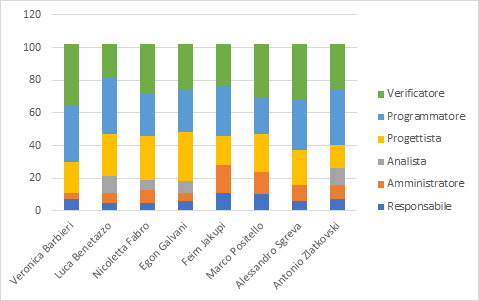
\includegraphics[width=0.7\textwidth]{./res/img/totaleRendicontate_po.png}
				\caption{Suddivisione oraria con il totale delle ore rendicontate}
			\end{figure}

		\newpage
		\subsubsubsection{Prospetto economico}
			Totale delle ore e costo per ciascun ruolo delle ore rendicontate:

			\rowcolors{2}{lightRowColor}{darkRowColor}
			\begin{longtable}{
				>{\centering}p{0.25\textwidth}
				>{\centering}p{0.05\textwidth}
				>{\centering\arraybackslash}p{0.15\textwidth} }

				\coloredTableHead
				\textbf{\color{white}Ruolo} &
				\textbf{\color{white}Ore} &
				\textbf{\color{white}Costo in \euro{}}
				\tabularnewline
				\endhead

				% Contenuto della tabella
				% Ruolo & Ore & Costo in \\
				Responsabile    & 57  & 1.710,00 \\
				Amministratore  & 73  & 1.460,00 \\
				Analista        & 33  & 825,00 \\
				Progettista     & 178 & 3.916,00 \\
				Programmatore   & 239 & 3.585,00 \\
				Verificatore    & 236 & 3.540,00 \\
				\textbf{Totale} & 816 & 15.036,00 \\

				\rowcolor{white}\caption {Prospetto dei costi totale delle ore rendicontate per ciascun ruolo} \\

			\end{longtable}

			\newpage
			% Grafico
			Rappresentazione grafica della distribuzione dei ruoli:
			\begin{figure}[h]
				\centering
				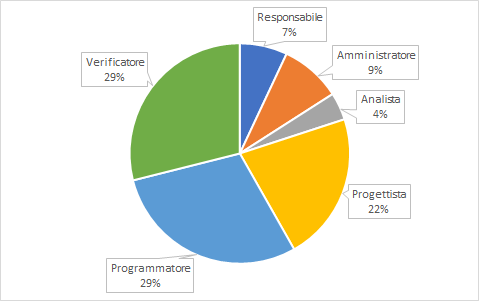
\includegraphics[width=0.7\textwidth]{./res/img/totaleRendicontate_pe.png}
				\caption{Suddivisione dei ruoli per il totale delle ore rendicontate}
			\end{figure}

\subsection{Conclusioni}
		Il costo preventivato totale per il progetto è di \textbf{\euro15.036,00}.
